\section{Experimental Evaluation}

We have evaluated our sensor planning solutions for gas emission monitoring in large environments, and conducted experiments in an indoor complex environment of size 000 $\times$ 00 m. Our robotic platform, as shown in Fig. 1, is Husky-200 which is running Robot Operating System (ROS), and equipped with an RMLD remote methane sensor and a pan-tilt unit. It is also equipped with the other sensors to navigation through the environment. In all the experiments, gas sampling was performed using sensing configurations of parameters $\phi = 270$\dg, and $r = 15$ m. 

%Fig. \ref{fig:exp} is an interface, which shows the details of one of the experiments. 
%One of the experiments is shown in Fig. \ref{fig:exp}. ... 






\begin{figure}[h!]
	\centering
	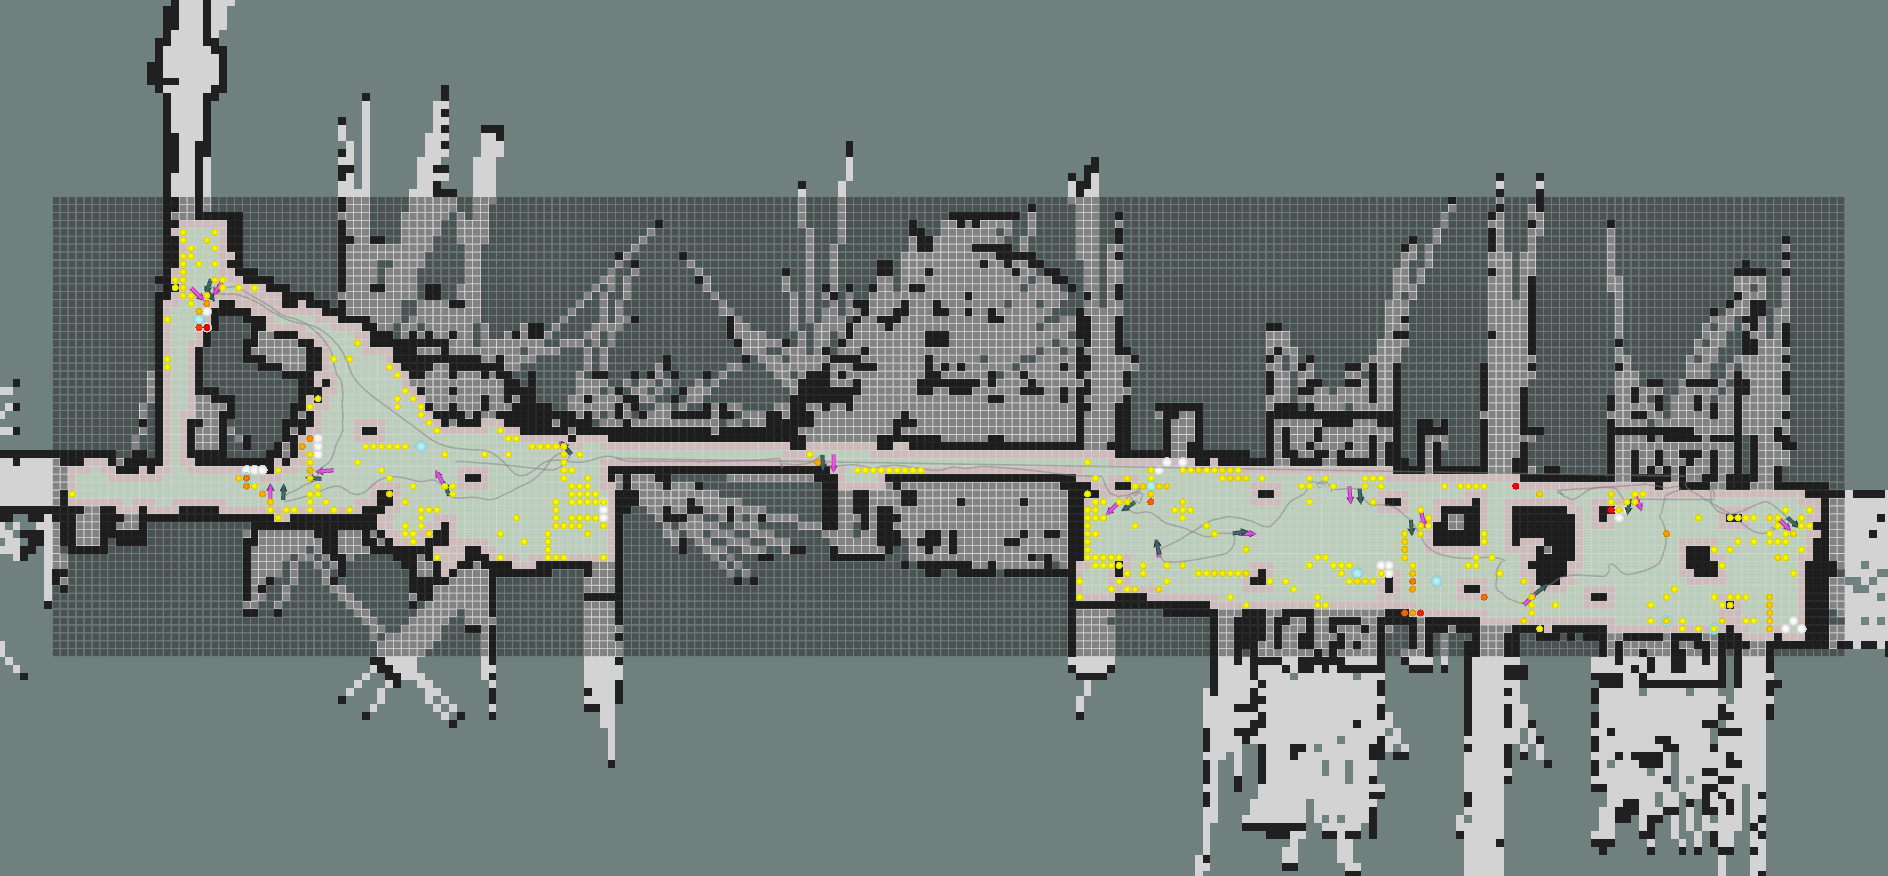
\includegraphics[trim={35 160 25 150}, clip,width=1\linewidth,angle=0]{fig/5-10-1se.png}
	%\vspace{1em}	
	\caption{A simulation scenario (to be replaced)}
	\label{fig:simulation}
\end{figure}



\begin{figure}[h!]
	\centering
	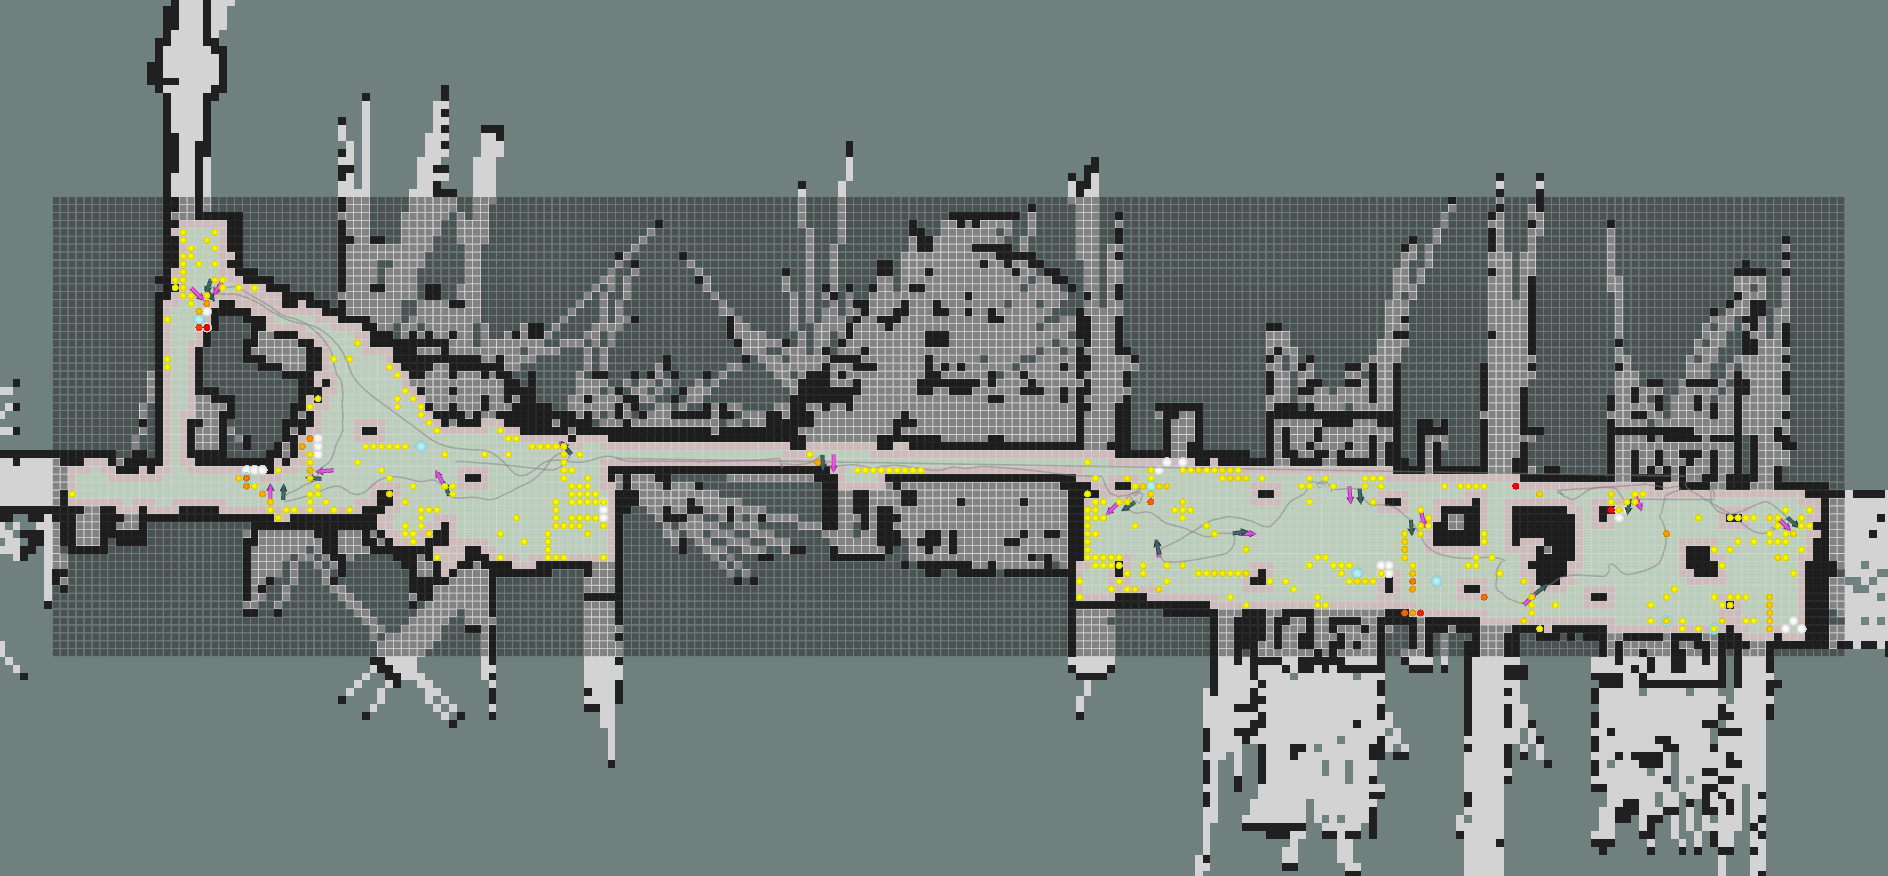
\includegraphics[trim={35 160 25 150}, clip,width=1\linewidth,angle=0]{fig/5-10-1se.png}
	%\vspace{1em}	
	\caption{A real-world scenario (to be replaced)}
	\label{fig:real-world}
\end{figure}

Fig. 1 shows the complete inspection process in a simulation scenario: the initial plan for the exploration task is shown in blue, which was later updated by an exploitation plan (in red) due to the detection of high gas concentrations present in the environment. In particular, configuration $c_1$ was executed for the exploration task, and $c_2$ and $c_3$ for the reconstruction purpose. After the exploitation process was completed at $c_3$, a new exploration plan was computed (in gray) and $c_4$ and $c_5$ were executed. The measurements collected for $c_5$ indicated another high concentration area, for which the exploitation was carried out by executing $c_6$ and $c_7$. Finally, an updated plan of $c_8,...,c_n$ was adapted for the exploration of the remaining uncovered area. It can noticed that the initially planned to the final executed configurations deviate from x to y, as the initial planned inspections was only for the exploration, and the new plans were adapted to exploit the environment while the inspection was carried out. %number of configurations deviates from x (initially planned exploration only) to y (the executed adapted plan), however, 
Therefore, the final inspection resulted not only a desired sensing coverage but also a high quality reconstruction of gas distributions.

Fig. 2 is an inspection of a real-world scenario, where configuration-poses are indicated with arrows. The configurations for the exploration and exploitation are marked in two different colors, and the final reconstruction of gas distribution is shown in yellow-to-red circles for low-to-high concentrations.

%\foreach \x in {01,02,03,04,05,06,07,08,09,10,11,12,13,14,15,16,17,18}
%{	
%	\begin{figure}[H]
%		\centering
%		\includegraphics[trim={25 160 25 150}, clip,width=1.1\linewidth,angle=0]{fig/\x.png}
%		%\vspace{1em}
%		%\label{fig:\x}
%		\caption{Reconstruction \#\x.}		
%	\end{figure}
%}
